\chapter{Апробация решения} \label{ch4}

\section{Оценка ExCodeAgent-MM} \label{ch4:sec1}

``Ядром'' предлагаемого решения ExCodeAct является агент кодогенерации ExCodeAgent-MM:
именно он в апробации использует бо'льшую часть спектра предлагаемых инструментов. 

Ввиду специфики задачи (а именно создание MAS для работы \textit{с внутренними} 
инструментами), использование публичных бенчмарков для тестирования является в определенном
смысле нецелесообразным: важно оценить качество агента именно в применении внутренних
инструментов, информация о которых была малоизвестная LLM-моделям.

Потому ниже будет представлен полное изложение анализа предлагаемого решения и сравнения
его с аналогами в кодогенерации с использованием внешних источников.

\subsection{ClearML-bench - система корректности работы с окружением} \label{ch4:sec1:subsec1}

В рамках тестирования корректности работы системы был создан собственный  
бенчмарк ClearML-bench, содержащий 15 вопросов-сценариев для взаимодействие 
с окружением в различных вариациях: работа с датасетами (создание, загрузка и выгрузка, 
анализ содержмого), работа с данными (преобразования, визуализации и сохранение) и прочее.
Полный список вопросов представлен в Приложении №\footnote{добавить приложение}. 

Принцип, по которому происходит тестирование, описать просто: каждое задание направлено на 
определенный набор взаимодействий с окружением (будь то файлы на локальном
хранилище, датасеты в системе ClearML). Сначала, перед запуском агента кодогенерации,
производится оценка окружения - так формируется начальное, $t_0$ описание окружения. 
Описание окружения состоит из содержимого ожидаемой рабочей директорией агента, с которой
предполагается работа (файлы, директории), а также из содержимого самого ClearML: какие
датасеты и задания на текущий момент там находятся. После этого производится запуск
агента кодогенерации с последующим снятием конечного описания окружения $t_1$. Поскольку
все представленные выше элементы описания окружения можно представить в виде множеств,
над которым определена операция разности, можно посчитать разность 
$\delta t = t_1 \backslash t_0$ и сравнить её с тем, какой результат ожидался. В случае
совпадения ожидания задание засчитывается и ставится 1 балл, в противном случае - 0 баллов.
Краткий график с работой представлен на \footnote{рисуночек тут с ClearML-bench}.

Хоть бенчмарк и назван в честь инструмента менеджмента данных и моделей ClearML, 
но тестирование охватывает сценарии с применением \textit{различных} инструментов: 
ClearML носит больше описательную характеристику окружения, 
с которым инструменты отчасти иногда взаимодействуют.

\subsection{Используемые инструменты} \label{ch4:sec1:subsec2}
В ходе тестирования принимало участие
4 внутренних кодовых инструмента-пакетов, выполняющие следующие роли:
\begin{itemize}
    \item ``cloudml\_manager'' - модификация Python SDK ClearML для 
автоматического структурирования артефактов деятельности лаборатории (датасетов, заданий, 
моделей) по проектам;
    \item ``deconvolution\_module'' - модуль с классами и статическими методами 
для работы с трехмерными изображениями и их улучшения при помощи алгоритма деконволюции;
    \item ``denoising\_module'' - модуль с классами и статическими методами 
для работы с трехмерными изображениями и их улучшения при помощи алгоритма денойзинга;
    \item ``biobert\_module'' - мокап-модуль с классами и статическими методами для
работы с сигналами активности мозга; использовался как дополнительный функционал в рамках
тестирования для оценки длины контекста и качества выбора нужного инструмента;
    \item ``spinetool\_module'' - мокап-модуль с классами и статическими методами для
работы с трехмерными моделями дендритных шипов; использовался как дополнительный 
функционал в рамках тестирования для оценки длины контекста и 
качества выбора нужного инструмента. 
\end{itemize}

Полный список используемых инструментов лаборатории представлен в 
Приложении №\footnote{сделать таблицу с инструментами}.

\subsection{Результаты кодогенерации} \label{ch4:sec1:subsec3}

Тестирование ExCodeAgent-MM производилось в полном описании, которое приводилось в главе 
\ref{ch3}: с использованием Coarse-Fine RAG и кодовой LLM Codestral-latest. Данная модель
больше обучена для генерации и работы с кодом, потому её использование здесь вполне логично.

Кроме того, для сравнения было проведено тестирование как на различных ретриверах, 
работающих по принципу косинусального сходства (с семантическим и рекурсивным 
разбиением документации на блоки),а также с различными LLM-моделями, список который ниже:
\begin{itemize}
    \item Mistral-Large-instruct - большая модель семейства Mistral общего назначения;
    \item Mistral-Small-instruct - маленькая модель семейства Mistral на 8B параметров;
    \item Mistral-Mini-instruct - самая маленькая модель семейства Mistral на 3B параметров;
\end{itemize} 
Все данные модели были запущены на удаленных вычислительных мощностях, предоставляемые
самим Mistral по API.

В качестве измеряемых параметров, помимо числа баллов в бенчмарке ClearML-bench, были
еще время работы и количество использованных токенов.

\begin{figure}
    \center
	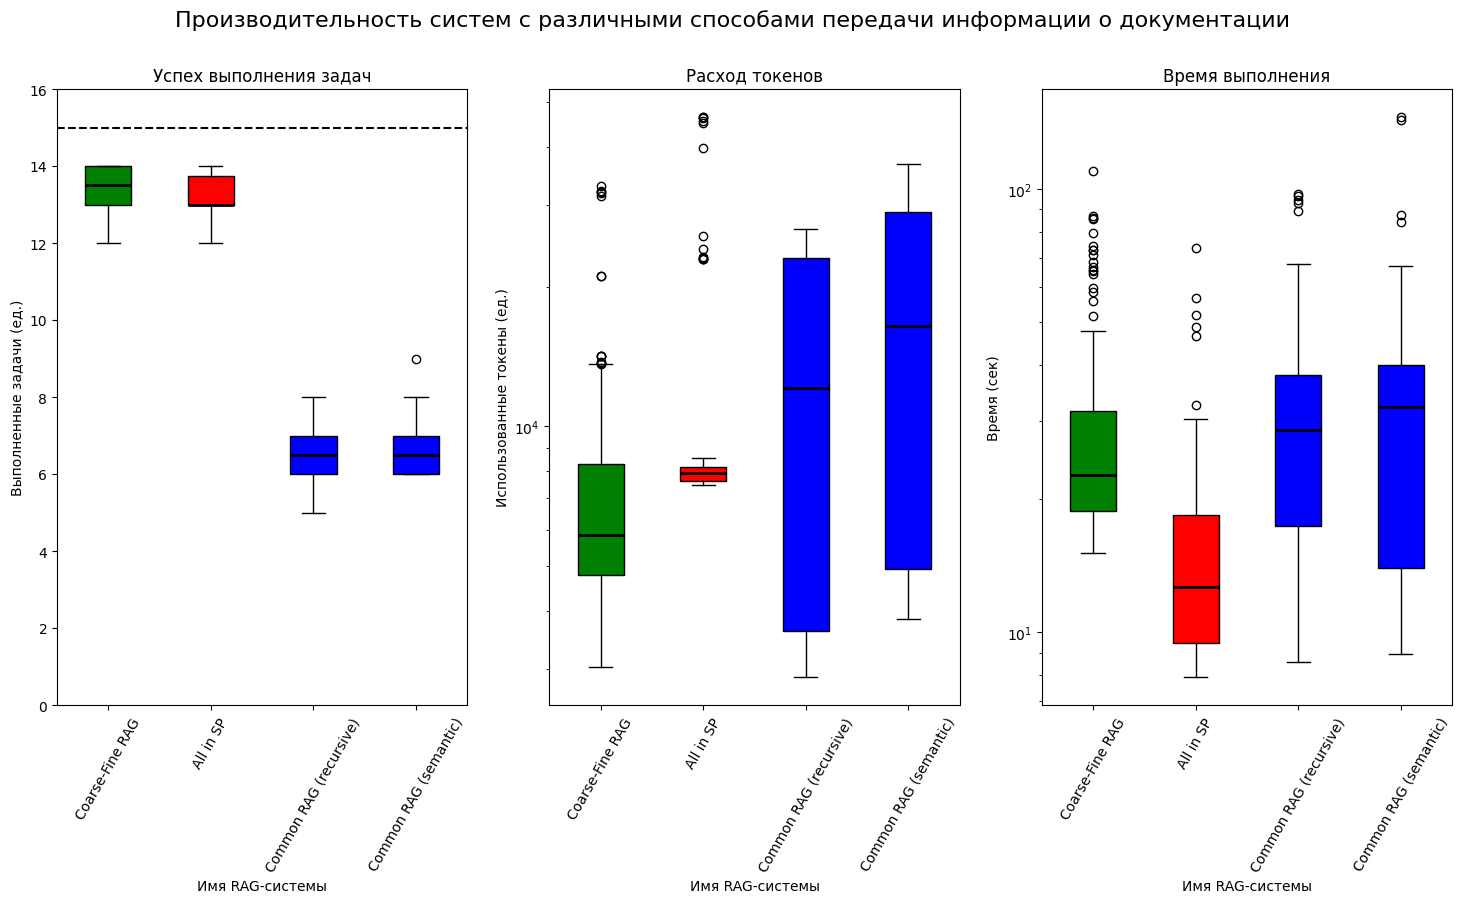
\includegraphics[scale=0.42]{sources/stats_1.png}
	\caption{Результаты работы ExCodeAgent-MM на различных ретриверах.} 
	\label{fig:ch4:rags}  
\end{figure}

На рисунке \firef{fig:ch4:rags} представлены результаты работы ExCodeAgent-MM на различных ретриверах. Кроме 
обычных ретриверов также приведены результаты работы в случае, когда использована подгрузка
документации всех инструментов в контекст модели. Как видно, количество токенов в случае
``coarse-fine RAG'' наименьшее, а число выполненных задач - наибольшее. Это свидетельствует
о том, что вся полезная информация для кодогенераций подгружается лучше в условиях 
структурированной организации, которые классические ретриверы не обеспечивают.

\begin{figure}
    \center
	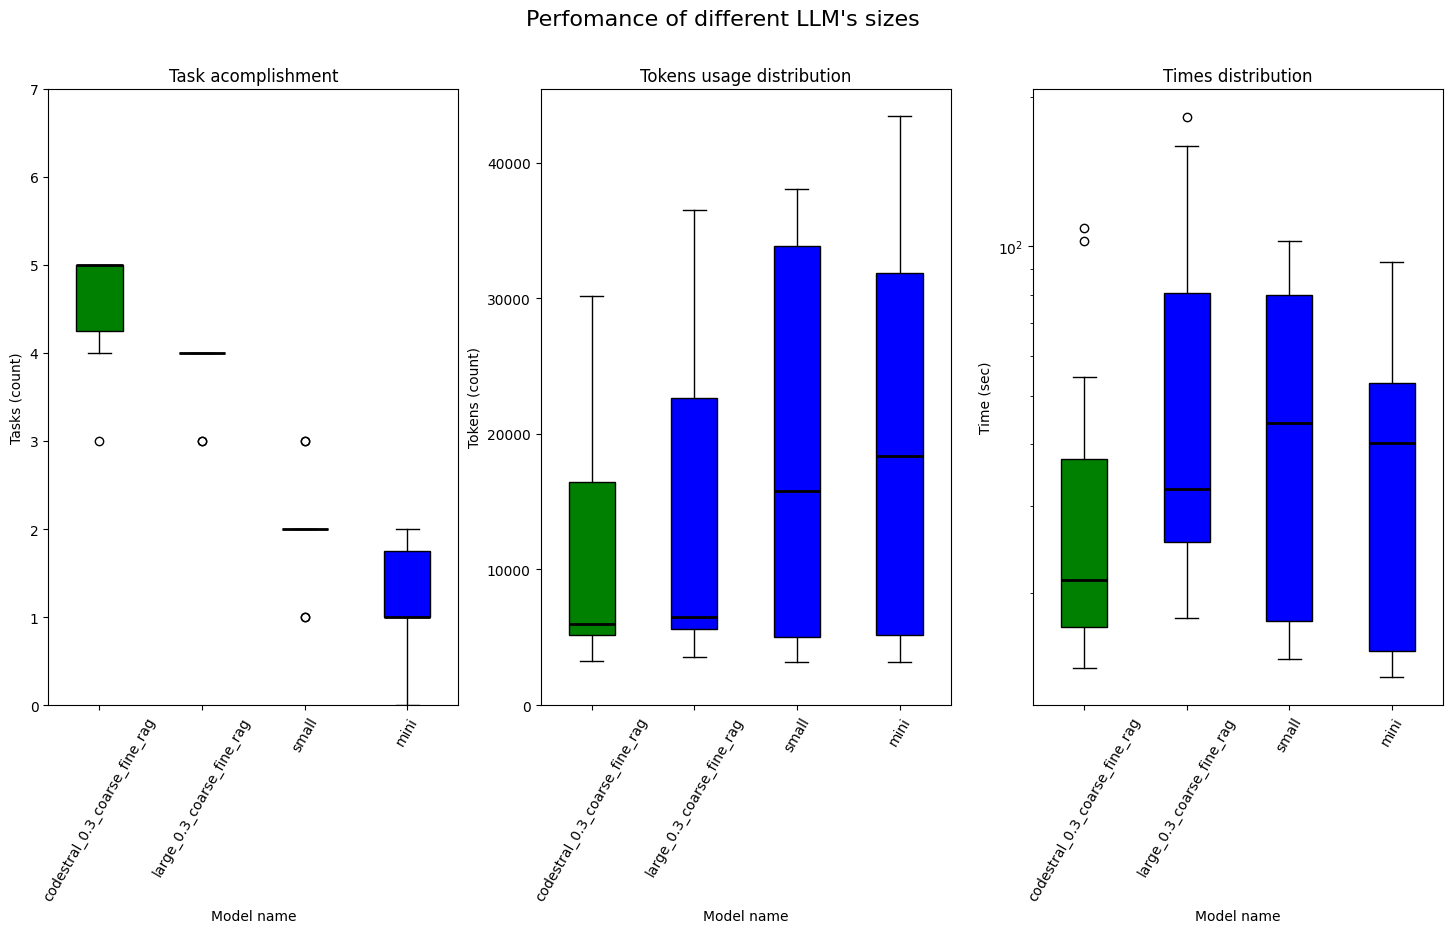
\includegraphics[scale=0.42]{sources/stats_2.png}
	\caption{Результаты работы ExCodeAgent-MM на различных моделях.} 
	\label{fig:ch4:llms}  
\end{figure}

На рисунке \firef{fig:ch4:llms} представлены результаты работы ExCodeAgent-MM на 
различных больших языковых моделях. Из графико видно, что использование как 
специализированной, так и большой модели общего назначения, практически одинаково сказываются
на числе решенных задач. Также стоит заметить, что число решенных задач по мере уменьшения 
числа обучаемых параметров модели также падают - малыми моделями решаются только 
простые задачи, в которых требуется вызов нескольких методов без построения логики программы
на основе циклов и условий.

% Но важно отметить следующее: решенные задачи
% малыми моделями - задачи, не связанные с ClearML PythonSDK (задачи на деконволюцию, 
% построение графиков и другие). 
% По мере уменьшения числа параметров падает понимание того, как именно
% работать с малорепрезентативными библиотеками, как ClearML: в процессе кодогенерации 
% малыми моделями вызывались ``несуществующие'' методы у экземпляров классов ClearML. 
% Это лишний раз показывает необходимость подгрузки документаций даже малорепрезнта

Писать про важность работы с контекстами, даже для публичных тулов но которые редко используют:
привести кодогенерации где что то забывается и тд и тп. Можно вынести в приложения.
В приложения также можно вынести список тулов (таблицы), примеры промптов 
(как типа код-снипет).
Писать про экстраполяцию на другие методы (опционально - если успеются графики на другие 
LLM семейства).

\subsection{Оценка количества наблюдений с текстовой и с мультимодальностью} \label{ch4:sec1:subsec4}


Здесь можно привести примеры на тестовых задачах Kaggle в вопросах анализа табличных данных
- сколько выводов извлекается из только тестовой модальности при автозапуске и сколько 
при мультимодальной (с анализом "чартов"). Очевидно, что будет не меньше - но насколько больше
- лучше показать. (Опционально - если успеются цифры/графики).


\section{Прочие качественные результаты} \label{ch4:sec2}

Здесь секция просто про то, что нельзя померить, но что просто есть и что стоит упомянуть.

Написать про оставшиеся свойства - про сохранение контекста, про создание юпитер ноутбуков
про сохранение графиков в них и все такое.
